\documentclass{article}

\usepackage[utf8]{inputenc}
\usepackage[T1]{fontenc}
\usepackage{geometry}
\usepackage{xcolor}
\usepackage{graphicx}
\usepackage{subcaption}
\usepackage{verbatim}
\usepackage{amsmath,amssymb}
\usepackage{amstext}
\usepackage{amsthm}
\usepackage{steinmetz}
\usepackage{stackrel}
\usepackage{mathtools}
\geometry{a4paper}

\usepackage[english]{babel}
\frenchspacing

\counterwithin{figure}{section}
\counterwithin{table}{section}

\title{Ale's report}
\author{Alessandro Matteo Rossi}
\date{data}

\begin{document}
\maketitle




\tableofcontents

\clearpage

\section{Decoder}

After the inputs have been processed (added or subtracted), it is needed a decoder (see figure \ref{Decoder}) in order to convert the output from binary number to its decimal form. Considering that this 16-bit calculator allows the user to insert numbers within the range (INSERIRE IL RANGE CAZZO), the operative boundary of this calculator is (INSERIRE).

\vspace{3mm}

The largest number that can be shown as result is around $\pm$INSERIER (+INSERIER or -INSERIER, to be exact), both positive and negative. So the decoding circuit needs to have 6 led displays for the digits and one extra display for the sign.

\vspace{3mm}

We decided to operate the binary-decimal conversion with the so called "double dabble" circuit, that will be explained later in the report. Nevertheless this was not the main problem. The double-dabble converts positive numbers perfectly, but not negative ones. The major issue was to adapt this circuit to work with both positive and negative numbers. 

The representation of the negative binary numbers follows the "two's complement" rule. It means that taken a B number of bits, all the numbers that can be represented with a 0 in the $B-1$ position are considered positive, otherwise they are negative. This allows to split the 17 bits available in two sets of 16 bits, and so it is possible to have the range described above.

\begin{figure}[h]
    \centering
    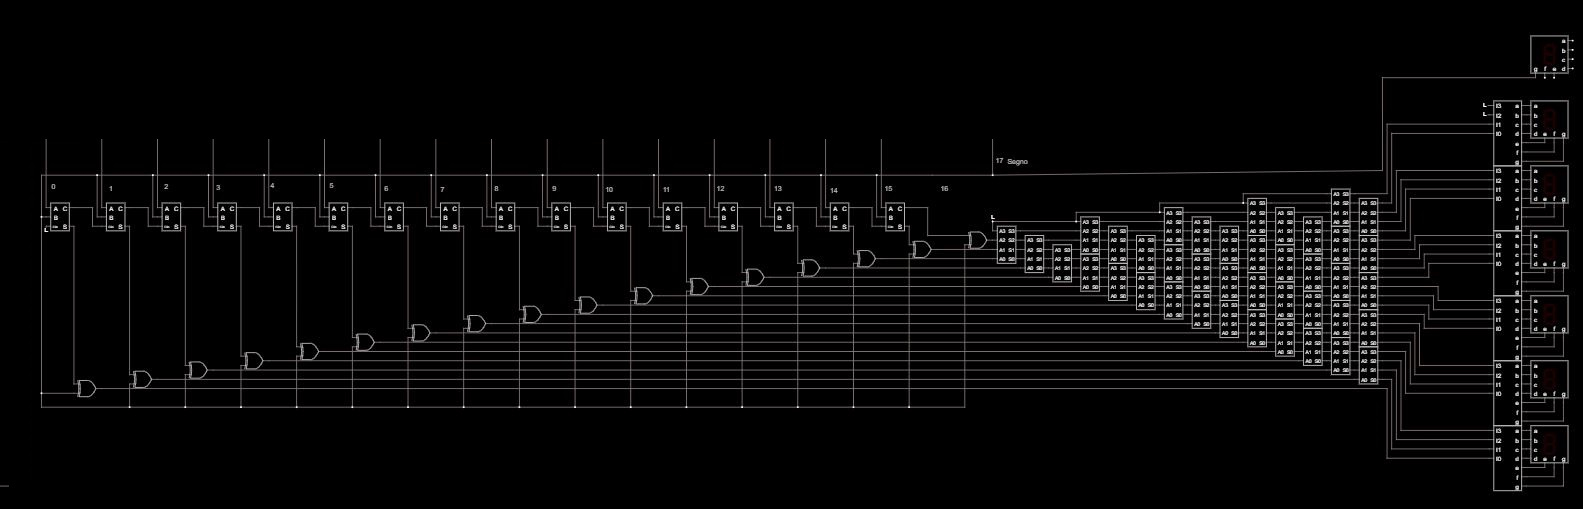
\includegraphics[scale=0.43]{SC_Decoder.JPG}
    \caption{Picture of the decoder}
    \label{Decoder}
  \end{figure}

\subsection{About the number sign}

The number sign has to be taken into account before converting the number into its decimal form. The number is a 16-bit binary, as already said, and it has one extra bit for the sign, the 16th bit.

First of all, we remember that if we consider a number $A$ written in binary form, its opposite is
\[-A=NOT(A)+1\]

This part of the circuit (represented in figure \ref{Converter}) uses full-adders and XOR logic gates, components that got already discussed in the previous sections. After the processing of the operation between the two inputs, the first 16 bits reach the A input of a specific full adder (the green lines in figure \ref{Converter}), whereas the sign bit follows the red path.

This 16th bit reaches every B input of all the full adders, and also the XOR gates, that compare the result of the single full adders with the 16th bit. The sign bit is true (or 1) when the number is negative and 0 otherwise. This allows the full adders to sum 1, following the formula above, if the processing output is negative, whereas if it is positive the number just stays the same.

After this, the XOR gates, which table of truth is 
\begin{center}
\begin{tabular}{||c|c||c||}
    \hline
    A & B & A XOR B \\
    \hline
    0 & 0 & 0 \\
    \hline
    0 & 1 & 1 \\
    \hline
    1 & 0 & 1 \\
    \hline
    1 & 1 & 0 \\
    \hline
\end{tabular}
\end{center}

give the final result, which will go to the double dabble. Considering the full adder output as "A" for the XOR, and the sign bit as "B", it is possible to deduct that when the sign is false (so the processing output is positive) the XOR gates do not modify the full adder output (which do not work too, considering that their "B", the sign bit, is false as well). When the XOR "B" is true (so the processing output is negative), the XOR gives the opposite of its "A" as output.

\begin{figure}[h]
    \centering
    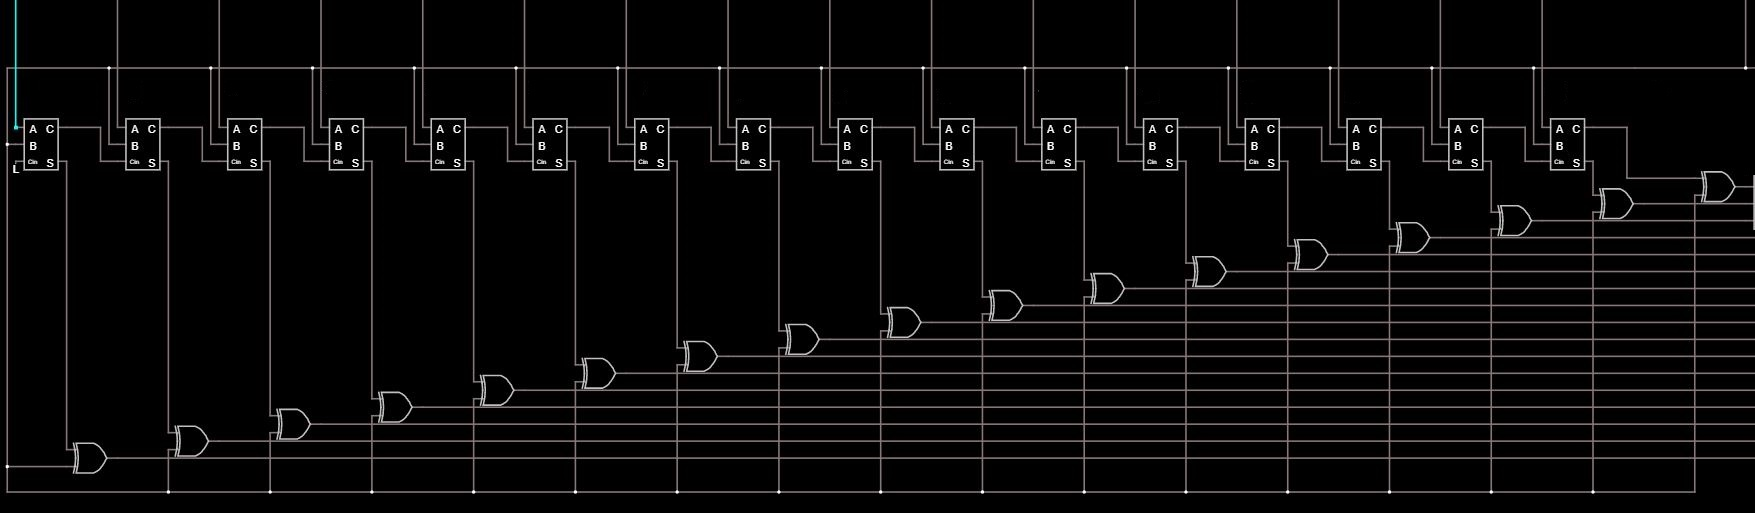
\includegraphics[scale=0.43]{SC_Converter.JPG}
    \caption{Picture of the first part of the decoder}
    \label{Converter}
  \end{figure}

\subsection{Double dabble}

This second part of the decoder is reached by the number that needs to be converted into decimal form. 

The entire circuit relies on an algorithmic process based on the concept of "shift and add 3", which is the name of the component that mostly populates figure \ref{DoubleDabble}.

This algorithm takes a binary number and after having processed it gives an output divided into smaller parts composed of 4 bits each. Everyone of these parts will be then elaborated by 7 segment decoders and represent a single digit of the decimal number. The 7-segment decoders are obviously connected to 7-segments led displays, that can be seen on the right side of figure \ref{DoubleDabble}.
\begin{figure}[h]
    \centering
    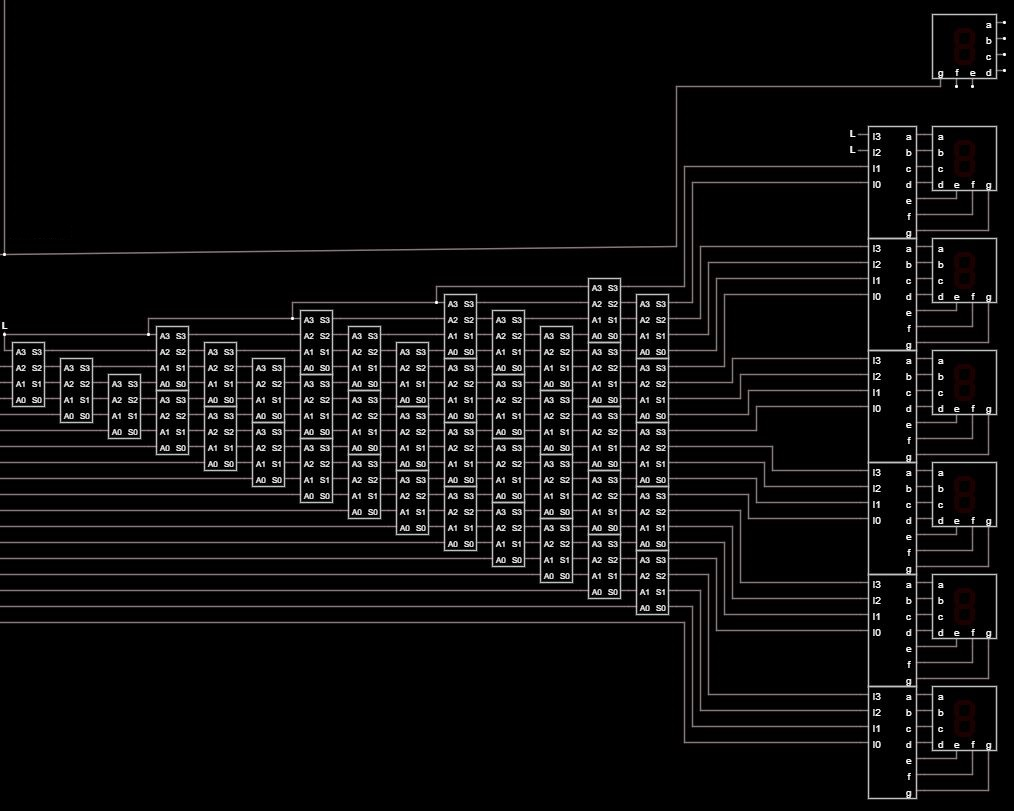
\includegraphics[scale=0.43]{SC_DoubleDabble.JPG}
    \caption{Picture of the double dabble, the second part of the circuit}
    \label{DoubleDabble}
  \end{figure}


\section{Real calculator}

\end{document}